\documentclass[10pt,a4paper]{article}
\usepackage[utf8]{inputenc}
\usepackage{amsmath}
\usepackage{amsfonts}
\usepackage{amssymb}
\usepackage{graphicx}
\author{Ricardo Arango Giraldo}
\title{Prueba de selección en Rappi}
\begin{document}
\maketitle
	El equipo de operaciones de Rappi está interesado en predecir qué órdenes tienen más probabilidades de ser cancelados ya que no son lo suficientemente atractivos para los mensajeros. Para resolver este problema, tenemos una muestra de pedidos creados en septiembre de 2017.\\
	Su objetivo es utilizar este conjunto de datos para ayudar a Rappi a comprender qué factores influyen si un servicio es tomado y ofrecer recomendaciones para tomar acciones basadas en sus ideas para mejorar la operación de Rappi.
	\section{Exploración}
		\begin{figure}[h]
			\centering
			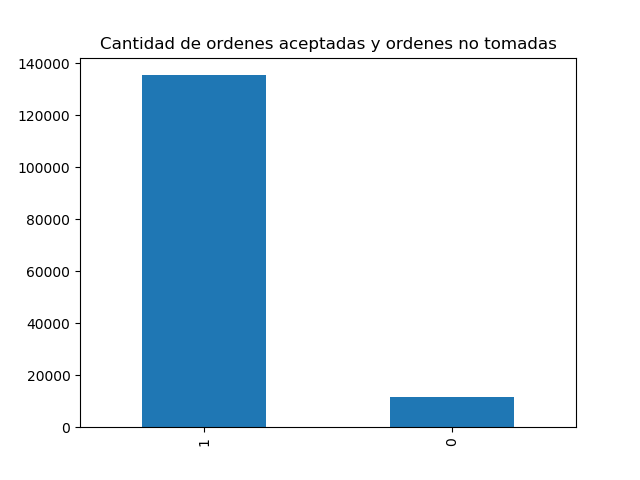
\includegraphics[width=0.5\textwidth]{../Img/Figure_1}
		\end{figure}
		
		\begin{figure}[h]
			\centering
			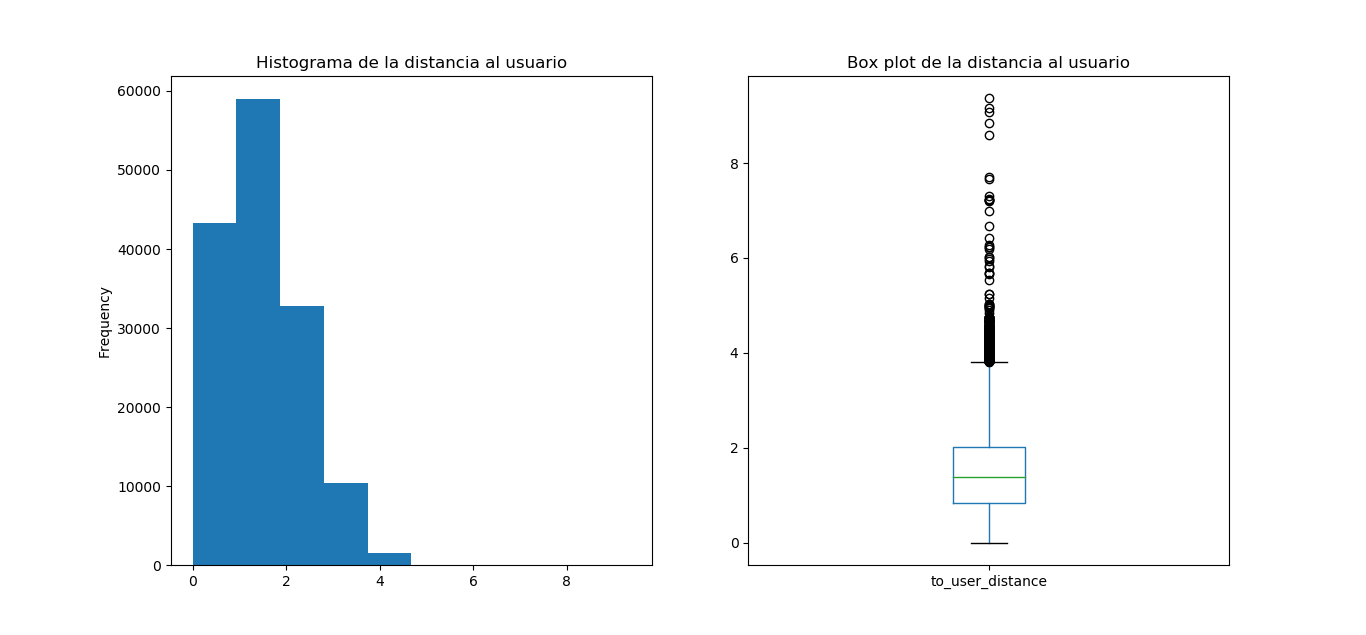
\includegraphics[width=0.5\textwidth]{../Img/to_user_distance}
		\end{figure}
	
		\begin{figure}[h]
			\centering
			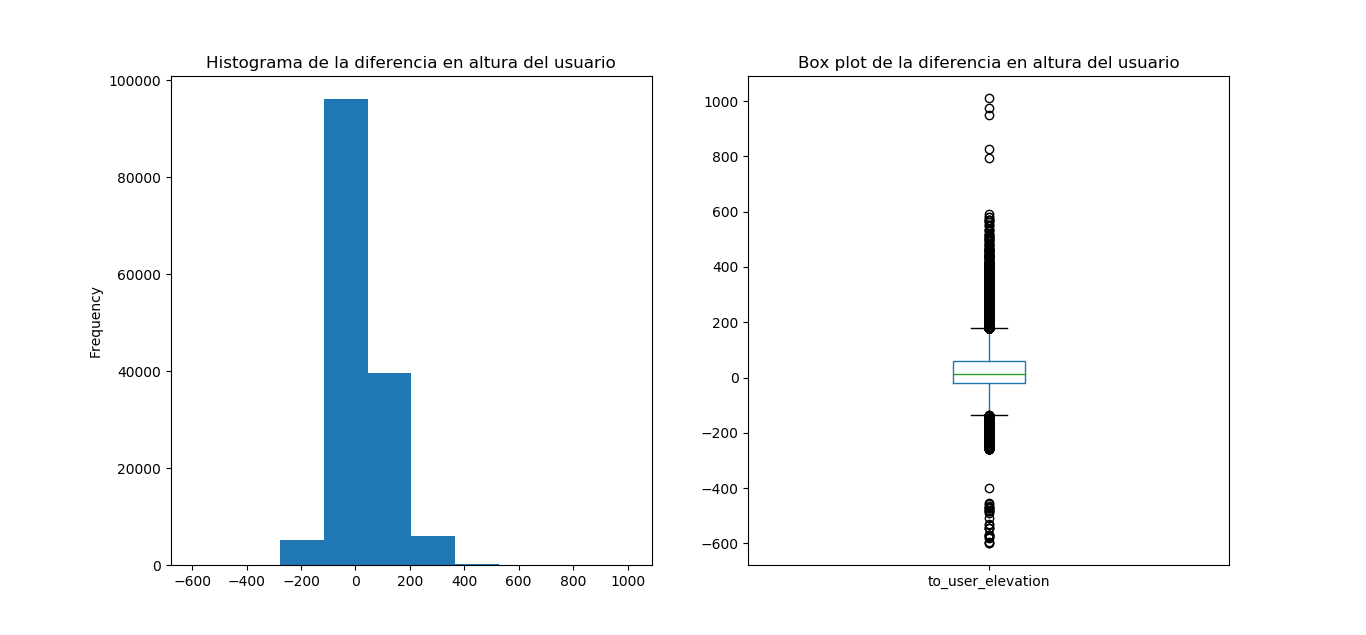
\includegraphics[width=0.5\textwidth]{../Img/to_user_elevation}
		\end{figure}
	
		\begin{figure}[h]
			\centering
			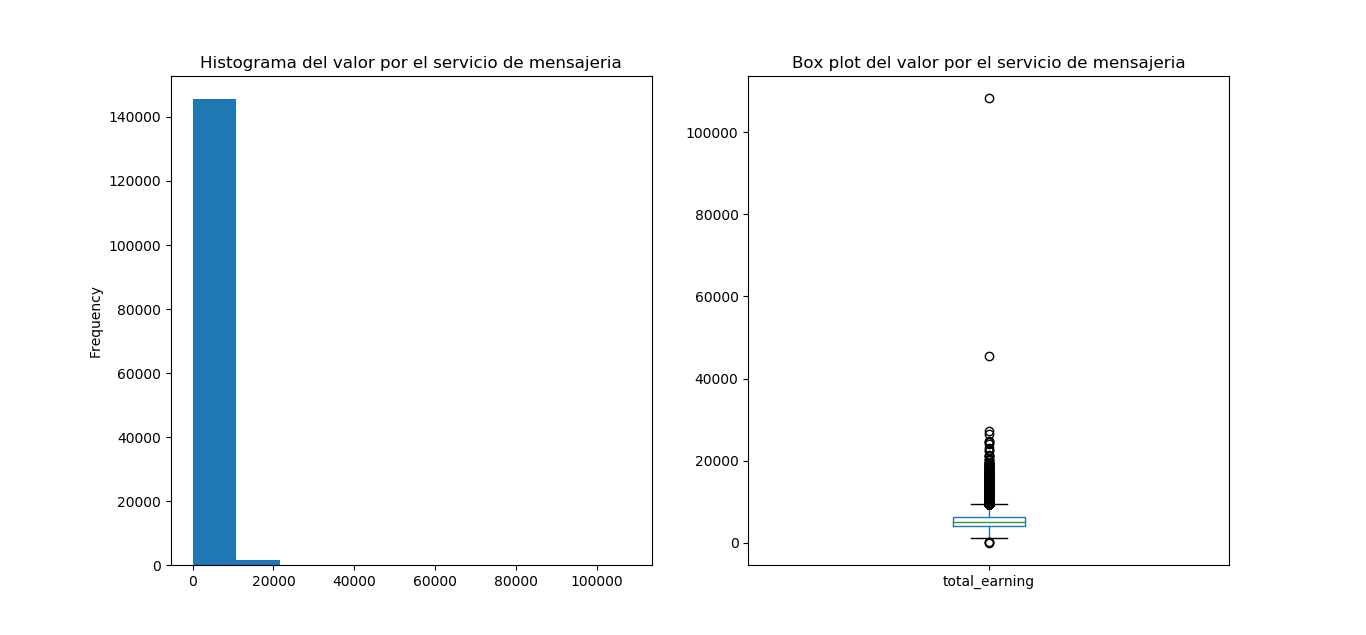
\includegraphics[width=0.5\textwidth]{../Img/total_earning}
		\end{figure}
	\section{Recomendaciones}
		\begin{figure}[h]
			\centering
			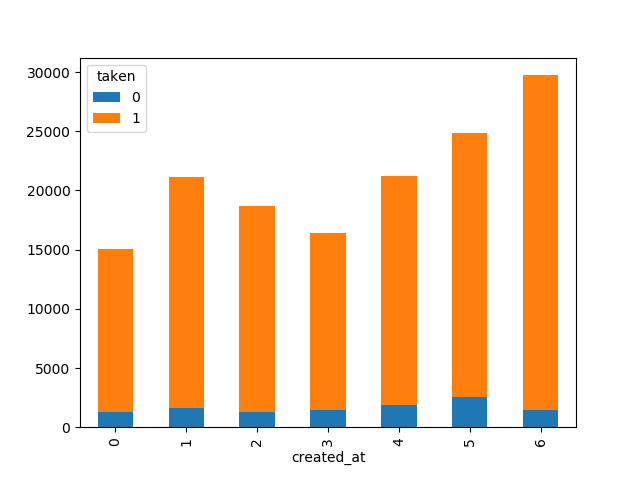
\includegraphics[width=0.5\textwidth]{../Img/Figure_2}
		\end{figure}
	
		\begin{figure}[h]
			\centering
			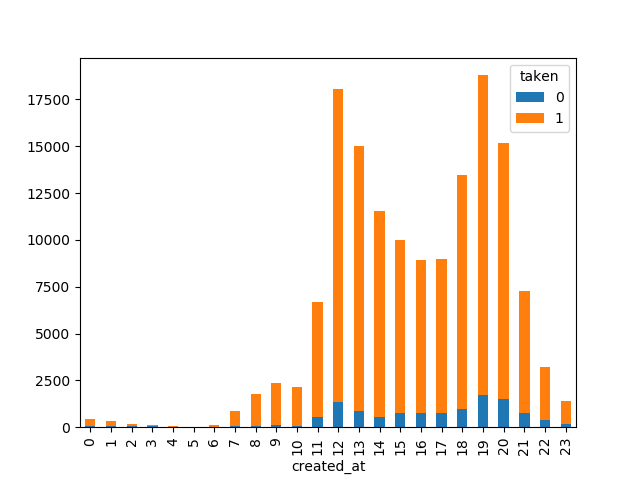
\includegraphics[width=0.5\textwidth]{../Img/Figure_3}
		\end{figure}
	
		\begin{figure}[h]
			\centering
			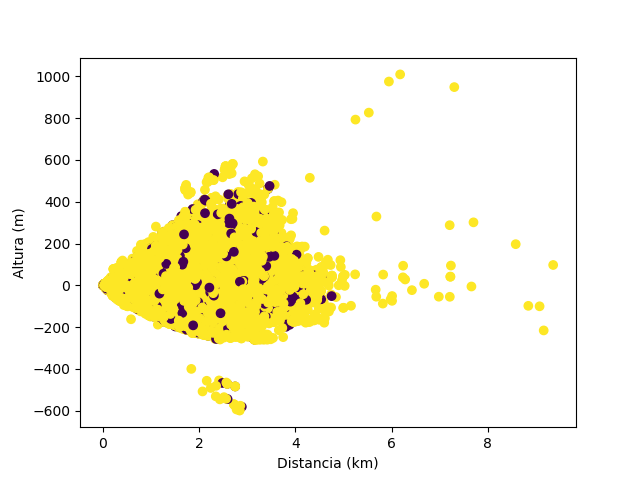
\includegraphics[width=0.5\textwidth]{../Img/Figure_4}
		\end{figure}
	
		\begin{figure}[h]
			\centering
			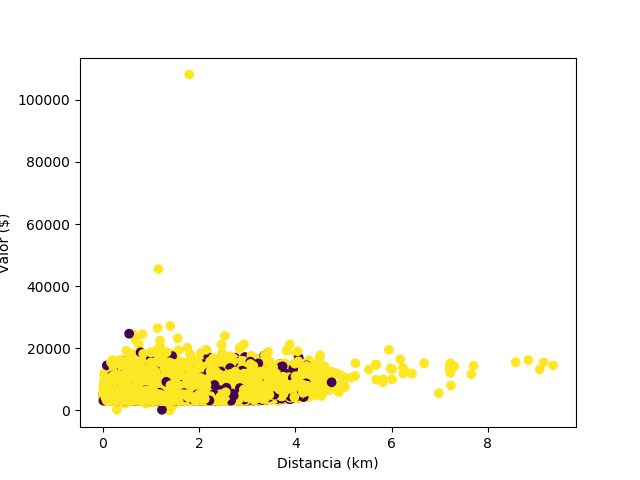
\includegraphics[width=0.5\textwidth]{../Img/Figure_5}
		\end{figure}
	\section{Modelo}	
		\begin{figure}[h]
			\centering
			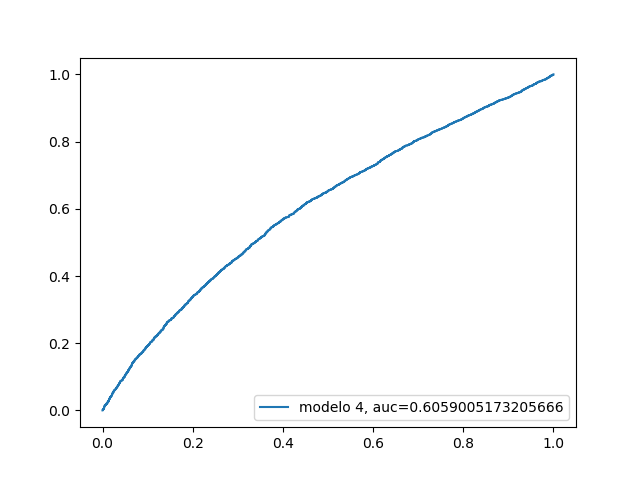
\includegraphics[width=0.5\textwidth]{../Img/curvaRocModelo4 }
		\end{figure}
\end{document}